\documentclass{article}

\usepackage{graphicx}
\usepackage{tikz}
\usepackage{tikzsymbols}
\usetikzlibrary{calc,patterns,shapes.geometric}
\pagestyle{empty}
\usepackage[margin=0pt]{geometry}
\geometry{papersize={14in,12in}}

\def\centerarc[#1](#2)(#3:#4:#5){\draw[#1] ($(#2)+({#5*cos(#3)},{#5*sin(#3)})$) arc (#3:#4:#5);}

\begin{document}
	\begin{figure}
		\centering
		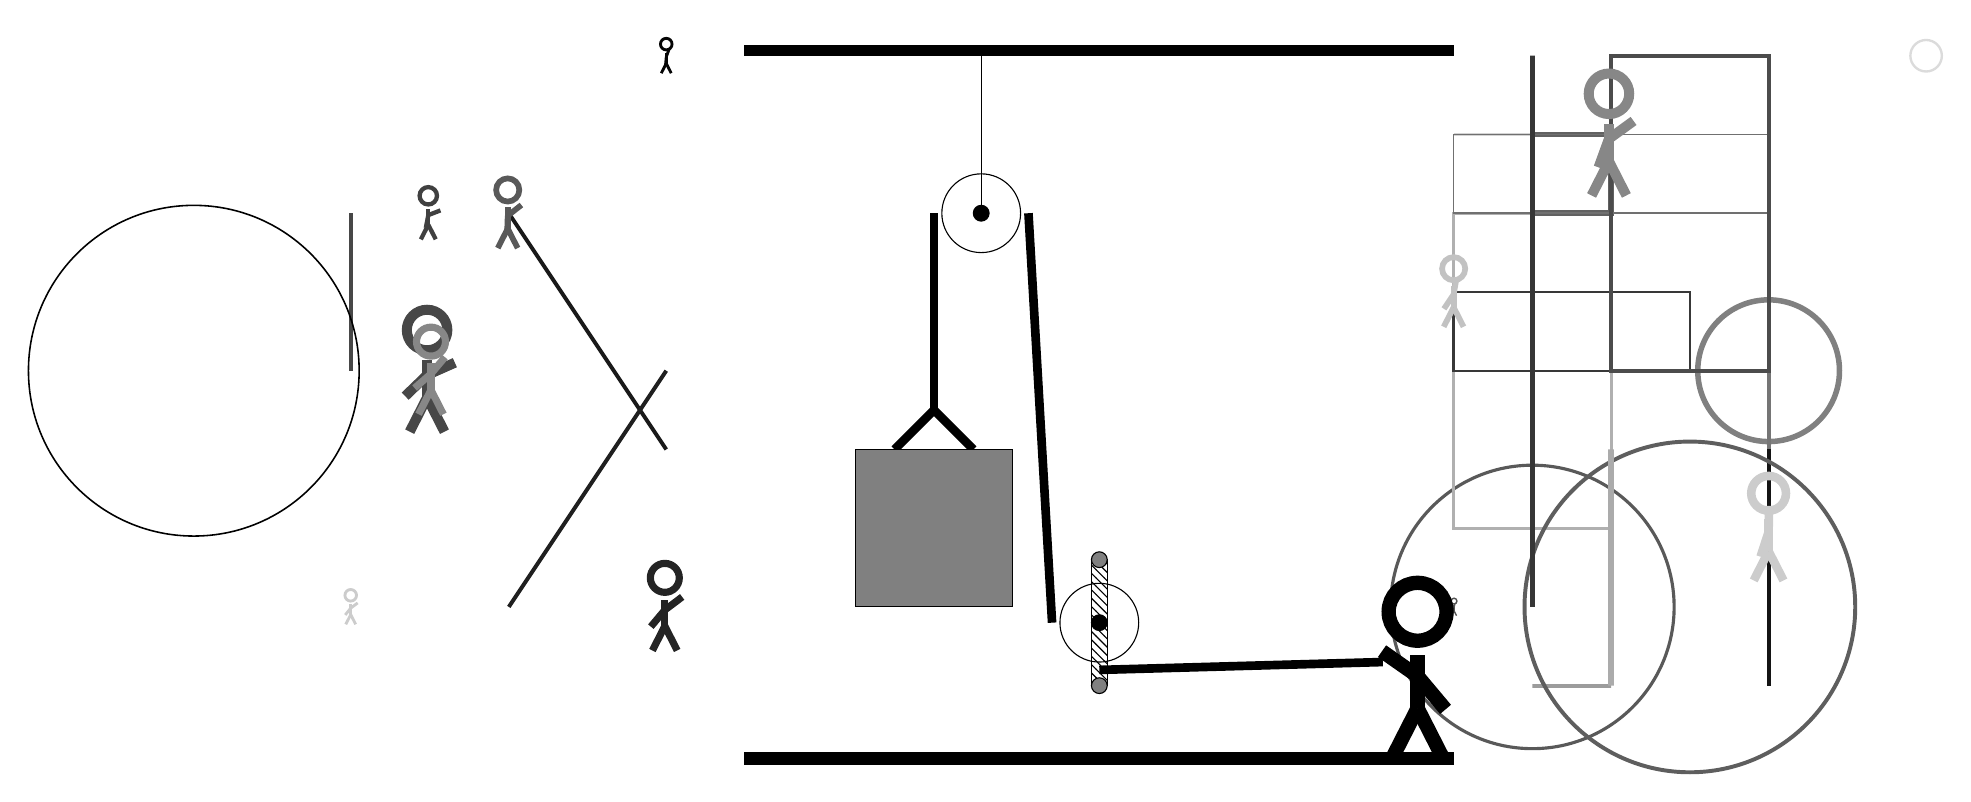
\begin{tikzpicture}
			%%%%% START %%%%%
			
			\draw[fill=black] (-2, 9) rectangle (7, 9.125);
			
			\draw (1, 7) circle (0.5);
			\draw[fill=black] (1, 7) circle (0.1);
			\draw (1, 9) -- (1, 7);
			
			\draw[fill=white](2.5, 1.8) circle (0.5);
			\draw[fill=black] (2.5, 1.8) circle (0.1);
			\draw[pattern=north west lines, pattern color=black] (2.4, 2.6) rectangle (2.6, 1.0);
			\draw[fill=black!50] (2.5, 2.6) circle (0.1);
			\draw[fill=black!50] (2.5, 1.0) circle (0.1);
			
			\draw [line width=0.7mm, color=black!50](11, 5) circle (0.9);
			
			\draw[line width=0.5mm, color=black!54](11, 6) -- (11, 2);
			\draw [line width=0.4mm, color=black!65](8, 2) circle (1.8);
			\draw[line width=0.5mm, color=black!92](11, 4) -- (11, 1);
			
			\draw[line width=0.5mm, color=black!17](7, 8) -- (8, 8);
			
			\node[line width=0.7mm, color=black!86] at (-3, 2) {\Strichmaxerl[5][50][37]};
			
			\draw[line width=0.5mm, color=black!39] (8, 1) rectangle (9, 1);
			\node[line width=0.6mm, color=black!72] at (-6, 5) {\Strichmaxerl[7][44][24]};
			\draw[line width=0.4mm, color=black!31] (9, 7) rectangle (7, 3);
			\draw[line width=0.5mm, color=black!90](-3, 4) -- (-5, 7);
			\draw[line width=0.7mm, color=black!62] (9, 8) rectangle (8, 7);
			\node[line width=0.4mm, color=black!68] at (7, 2) {\Strichmaxerl[1][33][78]};
			\node[line width=0.4mm, color=black!65] at (-5, 7) {\Strichmaxerl[4][88][38]};
			\node[line width=0.3mm, color=black!20] at (-7, 2) {\Strichmaxerl[2][51][37]};
			\draw[line width=0.2mm, color=black!56] (7, 8) rectangle (11, 7);
			\draw[line width=0.5mm, color=black!88](-5, 2) -- (-3, 5);
			
			\draw[line width=0.5mm, color=black!72](-7, 5) -- (-7, 7);
			\node[line width=0.4mm, color=black!98] at (-3, 9) {\Strichmaxerl[2][85][70]};
			\draw [line width=0.2mm, color=black!100](-9, 5) circle (2.1);
			
			\draw[line width=0.3mm, color=black!78] (7, 6) rectangle (10, 5);
			\node[line width=0.6mm, color=black!20] at (11, 3) {\Strichmaxerl[6][72][89]};
			
			\draw [line width=0.5mm, color=black!63](10, 2) circle (2.1);
			
			\node[line width=0.4mm, color=black!47] at (-6, 5) {\Strichmaxerl[5][41][50]};
			\draw[line width=0.7mm, color=black!79] (8, 2) rectangle (8, 9);
			\node[line width=0.2mm, color=black!75] at (-6, 7) {\Strichmaxerl[3][79][21]};
			\draw[line width=0.5mm, color=black!70] (9, 5) rectangle (11, 9);
			\node[line width=0.4mm, color=black!24] at (7, 6) {\Strichmaxerl[4][56][80]};
			\draw [line width=0.3mm, color=black!14](13, 9) circle (0.2);
			\node[line width=0.4mm, color=black!47] at (9, 8) {\Strichmaxerl[7][70][36]};
			\draw[line width=0.7mm, color=black!33] (9, 1) rectangle (9, 4);
			
			\draw[line width=1.1mm] (-0.1, 4.0) -- (0.4, 4.5) -- (0.9, 4.0);
			\draw[fill=black!50] (-0.6, 4.0) rectangle (1.4, 2.0);
			
			\draw[line width=1.1mm] (0.4, 7) -- (0.4, 4.5);
			\centerarc[line width=1.1mm](1, 7)(0:180:0.6);
			\draw[line width=1.1mm](1.6, 7) -- (1.9, 1.8);
			\centerarc[line width=1.1mm](2.5, 1.8)(180:270:0.6);
			\draw[line width=1.1mm](2.5, 1.2) -- (6.1, 1.3);
			
			\node at (6.5, 1.2) {\Strichmaxerl[10][-35][-50]};
			
			\draw[fill=black] (-2, 0) rectangle (7, 0.15);
			
			%%%%% END %%%%%
		\end{tikzpicture}
	\end{figure}	
\end{document}